\documentclass[compress, notes=hide]{beamer}
%\documentclass[compress, notes=hide,handout]{beamer}

\usepackage[english,norsk]{babel} %norske navn rundt omkring
\usepackage{lmodern}
\usepackage[T1]{fontenc} %Norsk tegnsetting (���)
\usepackage[latin1]{inputenc} %Norsk tegnsetting
\usepackage{amsmath,amsfonts,amssymb,mathrsfs} %matematikksymboler
\usepackage{algorithm, algorithmic}
\usepackage{amsthm} %for � lage teoremer og lignende.
\usepackage{bm} %fikser bold math-problematikken
%\usepackage[hang]{subfigure} %hvis du vil kunne ha flere figurer inni en figur
%\usepackage[small,bf,hang]{caption} %bestemmer format p� figurtekst
\usepackage{multirow}
\usepackage{graphpap}
\usepackage{pgf} %Tegning
\def\pgfex{ex}
%\usepackage{mathptmx}
%\usepackage{helvet}
%\usepackage{verbatim}

\setbeamertemplate{caption}[]
\setbeamertemplate{navigation symbols}{}
%\setbeamertemplate{footline}[page number]
\setbeamertemplate{footline}[frame number]
%\setbeamertemplate{caption}[numbered] 
\usecolortheme{default}
%\usetheme{Pittsburgh} %\usetheme{Singapore}
\setbeamertemplate{itemize item}[circle] %triangel p� 2-level-itemize (for 1-level brukt {itemize item})
\setbeamertemplate{itemize subitem}[triangle] %triangel p� 2-level-itemize (for 1-level brukt {itemize item})
\setbeamertemplate{section in toc}[circle]{} %Nummer i table of content
\setbeamertemplate{enumerate items}[circle] 
\setbeamertemplate{itemize subitem}[triangle] %triangel p� 2-level-itemize (for 1-level brukt {itemize item})
\setbeamercolor{itemize subitem}{fg=gray} %farge bullets

% For � skrive i default bl� farge:
% \textcolor[rgb]{0.2,0.2,0.7}{Blablabla-tekst}
%\newcommand{\hl}[1]{\textcolor[rgb]{0.2,0.2,0.7}{\emph{#1}}}
\newcommand{\hl}[1]{\textbf{#1}}
\newcommand{\hlb}[1]{\textcolor[rgb]{0.2,0.2,0.7}{#1}}
\newcommand{\sectionheader}{
    \usebeamerfont*{section number projected}%
    \usebeamercolor{section number projected}%
    \begin{pgfpicture}{-1ex}{-0.4ex}{1ex}{2ex}
      \color{bg}
      \pgfpathcircle{\pgfpoint{0pt}{.75ex}}{1.2ex}
      \pgfusepath{fill}
      \pgftext[base]{\color{fg}\thesection}
    \end{pgfpicture}\kern1.25ex
   \usebeamercolor[bg]{item projected}
    \Large{\insertsectionhead}
}

% FOR Å SKRIVE I DEFAULT, BLÅ FARGE:       \textcolor[rgb]{0.2,0.2,0.7}{Blablabla-tekst}



\title{Normal distribution} 
\author{Chi Zhang\\
	\footnotesize{Oslo Center for Biostatistics and Epidemiology}\\
	\footnotesize{Department of Biostatistics, UiO}\\
	\footnotesize{chi.zhang@medisin.uio.no}}
\date{MF9130 -- Introductory Course in Statistics\\
	31.01.2023}




\setbeamertemplate{navigation symbols}{}
%\setbeamertemplate{footline}[page number]
\setbeamertemplate{footline}[frame number]
\usecolortheme{default}
%\setbeamertemplate{background}[grid][step=0.25cm]%Rutenett


\begin{document}

\frame{\titlepage}

%DISP:
%SPSS: Hvordan tilpasse normalkurve

\section{Overview}

\frame{ 
\frametitle{Outline}
  \begin{block}{Aalen chapter 5, Kirkwood and Sterne chapter 5 and 6}
    \begin{itemize}
    \item Probability distributions for \hl{continuous data}
    \item \hl{The normal distribution}
    \item The normal \hl{approximation to binomial distribution}
    \end{itemize}
  \end{block}
}

\frame{ 
\frametitle{Introduction}
  \begin{block}{The normal distribution (or Gaussian distribution)}
    \begin{itemize}
    \item \hl{The most important probability distribution} in statistics
    \begin{itemize}
      \item Theoretical description of continuous data (probability density)
      \item Approximation of the distribution of a mean (central limit
        theorem)
      \item Approximation of probability distributions for discrete
        data \\
      \end{itemize}
      \begin{center} $\rightarrow$ Confidence intervals, statistical tests\end{center}
     \end{itemize}
    \begin{center}
      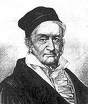
\includegraphics[height=0.20\textheight]{normal1.png}
    \end{center}
  \end{block}
}

\frame{ 
\frametitle{Probability distributions for continuous data}
  \begin{block}{Continuous variables}
    We distinguish between two important types of stochastic variables:
    counting variables and continuous variables \vspace{2mm}
    \begin{itemize}
    \item \hl{Counting variables}
    \begin{itemize}
    \item Discrete, possible to count
    \item Examples: \# of cases, \# of sixes, \# of boys
    \item For instance the Binomial distribution
     \end{itemize}
    \item \hl{Continuous variables}
    \begin{itemize}
    \item Continuous, measured on a scale
    \item Examples: height, cholesterol, annual salary
    \item For instance the normal distribution
     \end{itemize}
     \end{itemize}
  \end{block}
}

\frame{
\frametitle{}
\begin{block}{Example: birthweight of 189 newborns}
  \begin{figure}[ht]
    \begin{center}
      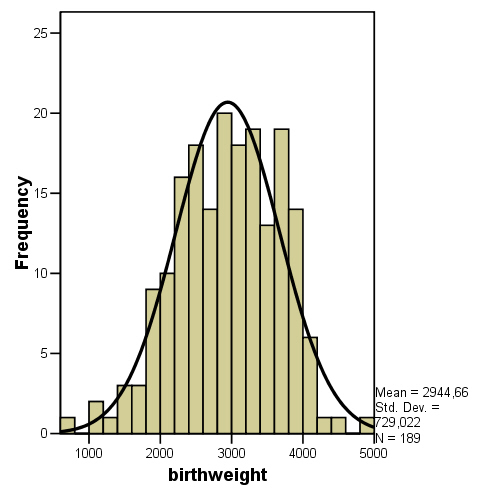
\includegraphics[height=0.70\textheight]{normaltina.png}
      %\caption{}
    \end{center}
  \end{figure}
  We observed a birthweight between 2000g and 2200g 10 times
\end{block}
}

\frame{ 
\frametitle{}
  \begin{block}{Probability density}
    As before we denote a stochastic variable as $X$, and a random
    possible value of the variable as $x$. \hl{The probability
      density for $\bm{X}$ is a function $\bm{f(x)}$} satisfying the following:
    \begin{itemize}
    \item $f(x) \geq 0 \text{ for all } x$
    \item The total area under the curve is 1
    \item $P(a \leq X \leq b)$ equals the area under the curve from $a$ to $b$
     \end{itemize}
  \begin{figure}[ht]
    \begin{center}
      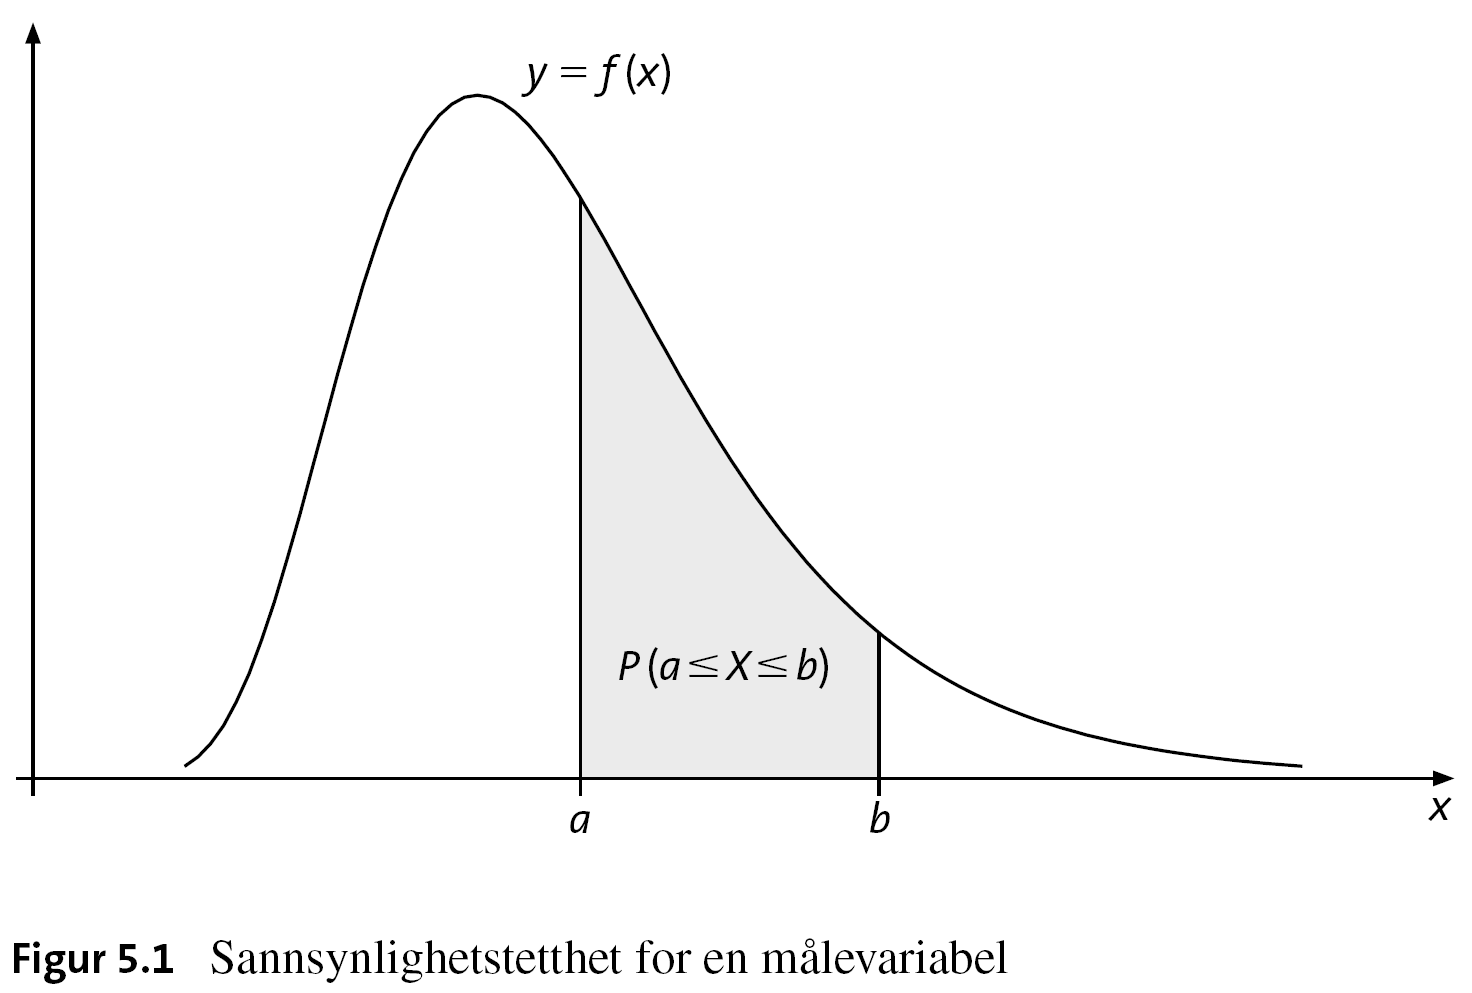
\includegraphics[height=0.45\textheight]{Figur5-1.png}
      %\caption{}
    \end{center}
  \end{figure}
  \end{block}
}

\frame{
\frametitle{}
\begin{block}{Example 1: height of a random 19 year male in Norway 1985}
  \begin{figure}[ht]
    \begin{center}
      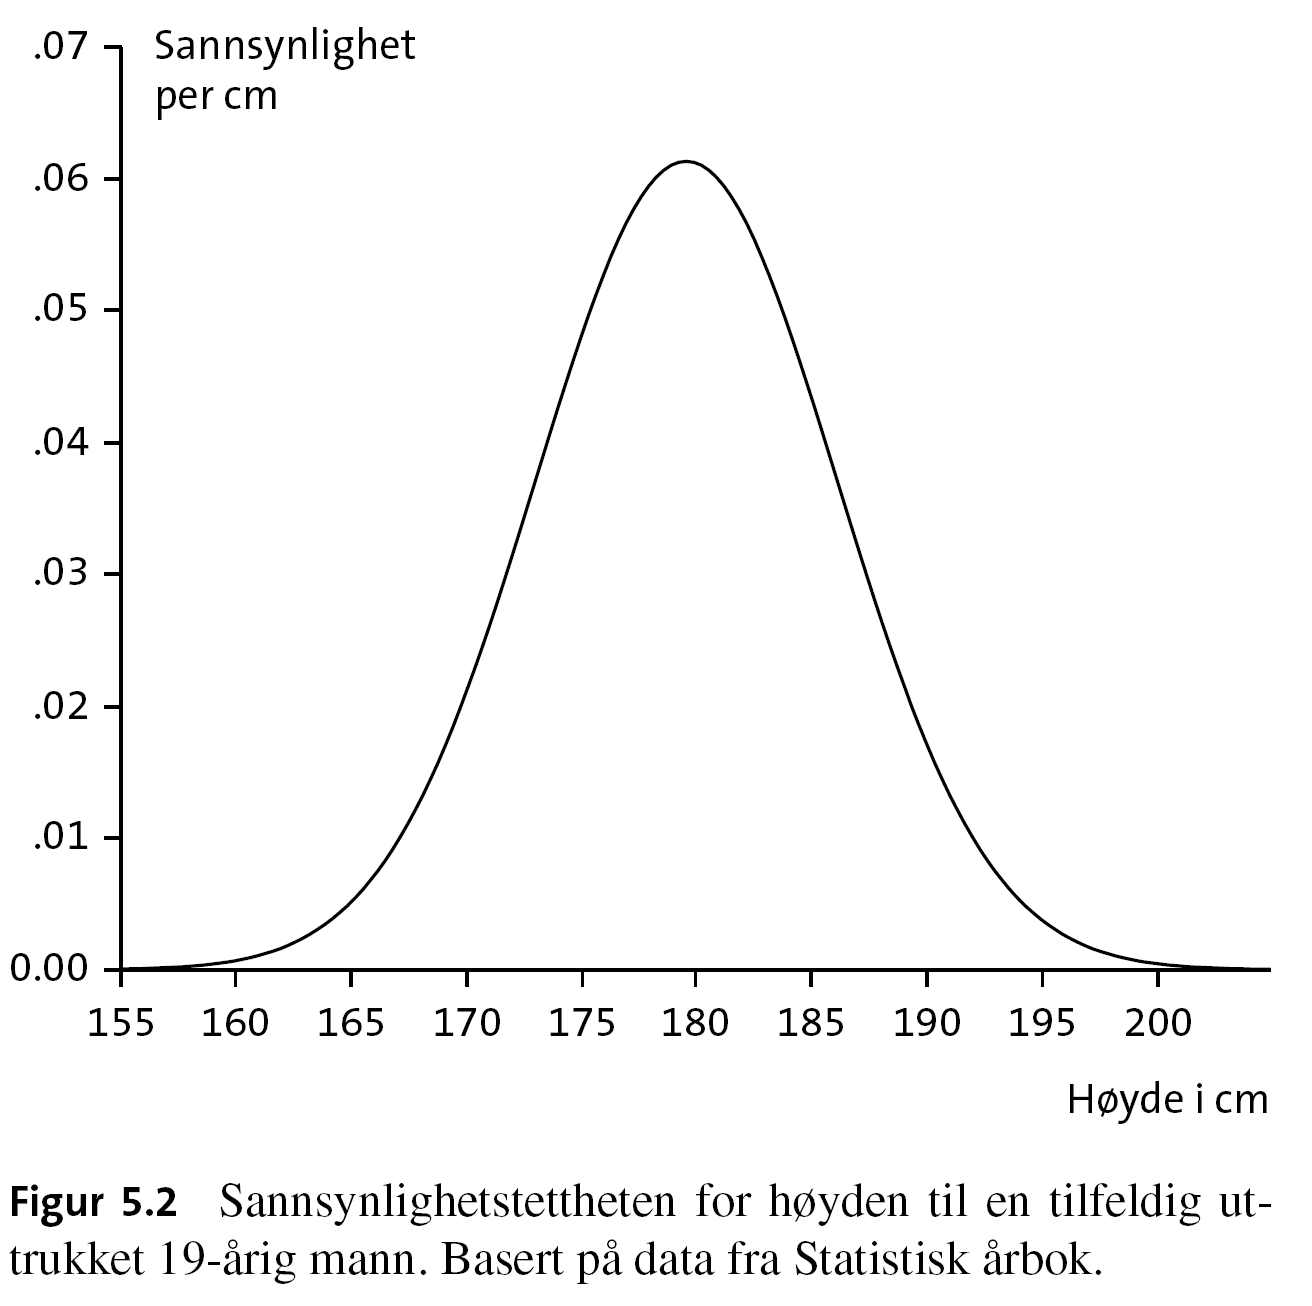
\includegraphics[height=0.65\textheight]{Figur5-2.png}
      %\caption{}
    \end{center}
  \end{figure}
\end{block}
}

\frame{
\frametitle{}
\begin{block}{Example 2: age distribution in Norway 1985}
  \begin{figure}[ht]
    \begin{center}
      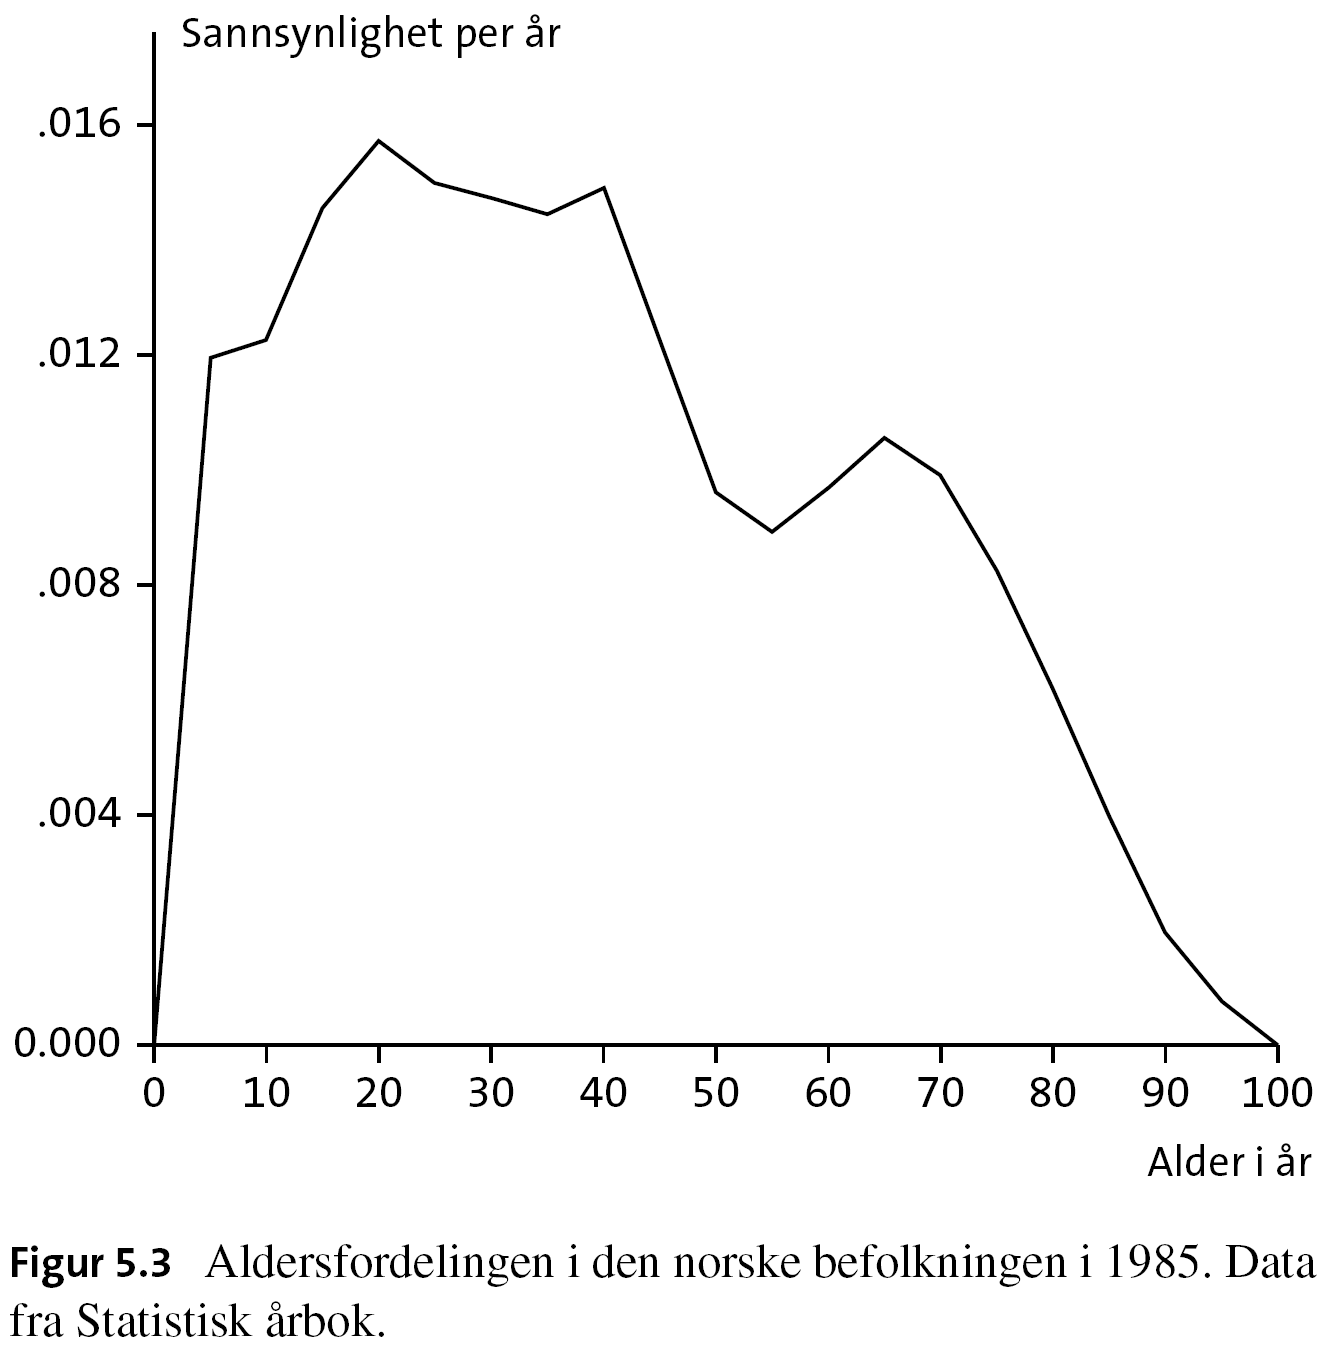
\includegraphics[height=0.65\textheight]{Figur5-3.png}
      %\caption{}
    \end{center}
  \end{figure}
    \begin{itemize}
    \item In general, different measure variables will give rise to different probability densities
     \end{itemize}
\end{block}
}

\frame{ \frametitle{The normal distribution}

  \begin{block}{Probability density function}
    \begin{itemize}
    \item $f(x) = \frac{1}{\sigma \sqrt{2 \pi}}
      \exp(-\frac{(x-\mu)^2}{2\sigma^2})$ \\ \vspace{2mm} where $\mu$
      is the mean, $\sigma$ the standard deviation and $\exp(a) = e^a$
     \end{itemize}
  \end{block}
}

\frame{ 
\frametitle{}
  \begin{block}{Properties of the normal distribution}
  \begin{figure}[ht]
    \begin{center}
      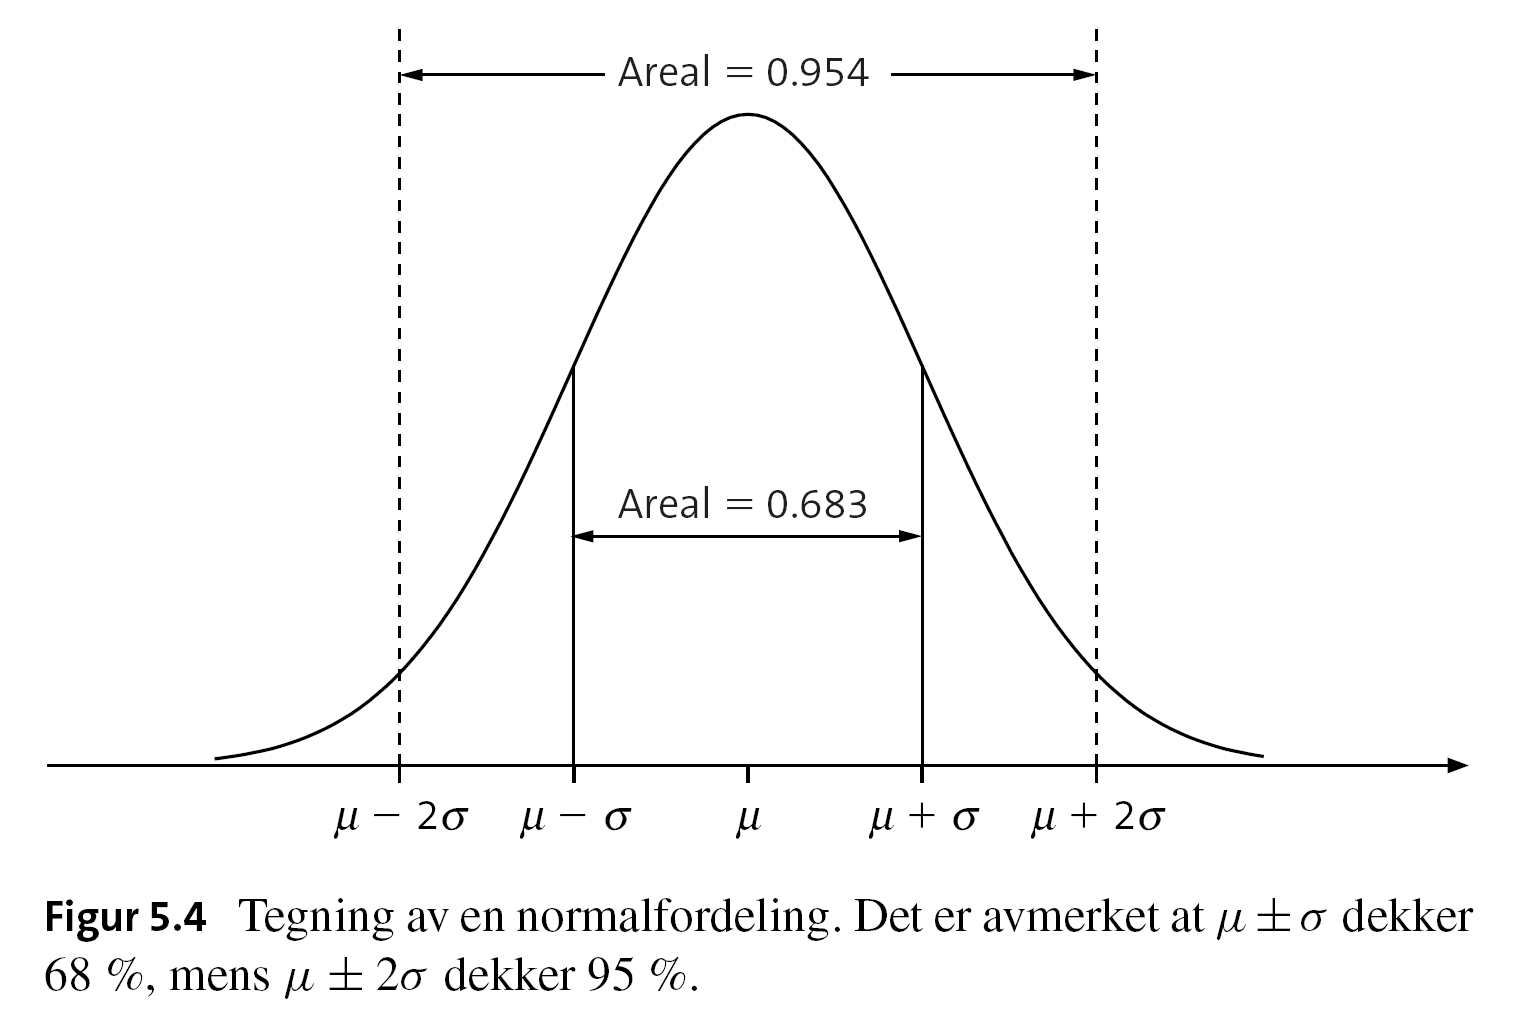
\includegraphics[height=0.60\textheight]{Figur5-4.png}
      %\caption{}
    \end{center}
  \end{figure}
    \begin{itemize}
    \item Symmetric bell-shape
    \item $\mu$ and $\sigma$ define the location and variation
    \item An interval with center at the mean value, going two standard
      deviations each way covers approx. 95\% of the distribution
     \end{itemize}
  \end{block}
}

\frame{
\frametitle{}
\begin{block}{Example: location $\mu$, variation $\sigma$}
  \begin{figure}[ht]
    \begin{center}
      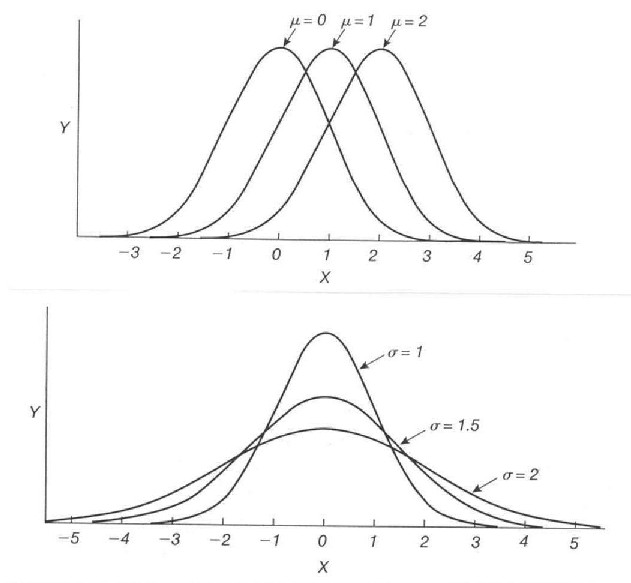
\includegraphics[height=0.7\textheight]{normaltina2.png}
      %\caption{}
    \end{center}
  \end{figure}
\end{block}
}

\frame{
\frametitle{}
\begin{block}{Possible normal density functions}
  \begin{figure}[ht]
    \begin{center}
      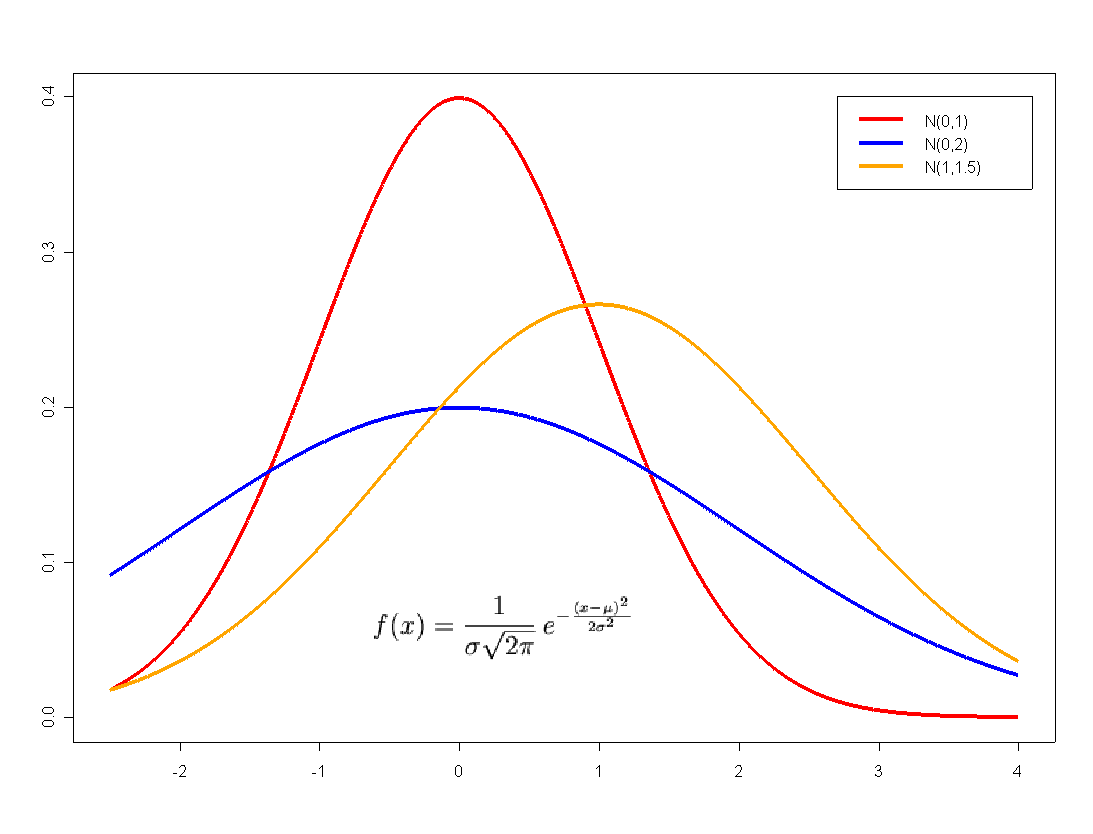
\includegraphics[height=0.8\textheight]{normaltina3.png}
      %\caption{}
    \end{center}
  \end{figure}
\end{block}
}

\frame{ 
\frametitle{}
  \begin{block}{The standard normal distribution}
    \begin{itemize}
    \item \hl{A normal distribution $\bm{N(\mu,\sigma)}$} with expectation $\mu = 0$ and variance $\sigma = 1$
    \item Any normal distribution $N(\mu,\sigma)$ can be transformed
      into \hl{a standard normal distribution $\bm{N(0,1)}$}...
    \item ... by substracting the mean and dividing by the standard deviation
     \end{itemize}
  \end{block}
}

\frame{ 
\frametitle{}
  \begin{block}{Transformation}
    \begin{itemize}
    \item If $X \sim N(\mu, \sigma)$, then $Y = \frac{X - \mu}{\sigma} \sim N(0,1)$
     \end{itemize}
    \begin{center}
      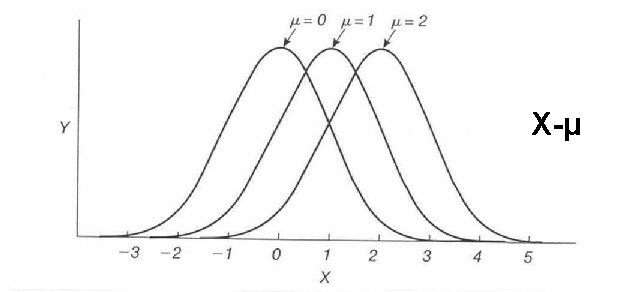
\includegraphics[height=0.4\textheight]{normal2.png}
      %\caption{}
    \end{center}
  \end{block}
}

\frame{ 
\frametitle{}
  \begin{block}{Example: birthweight of 189 newborns}
  \begin{figure}[ht]
    \begin{center}
      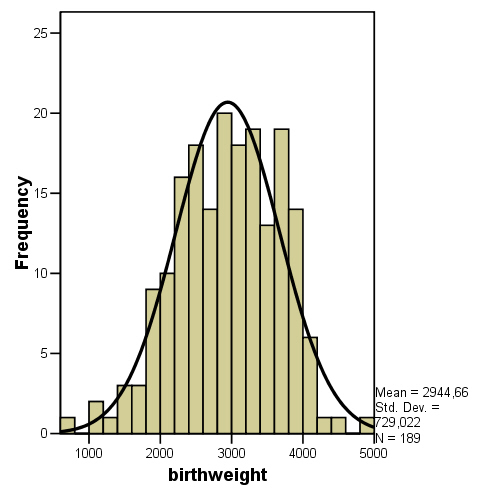
\includegraphics[height=0.50\textheight]{normaltina.png}
      %\caption{}
    \end{center}
  \end{figure}
    \begin{itemize}
    \item Estimates of $\mu$ and $\sigma$, respectively 2945g and 729g
    \item What is the proportion of weights > 4000g?
    \item P(X > 4000) = 1 - P(X $\leq$ 4000) = 1 - P($\frac{X-2945}{729} \leq 1.45$)
    \item Now, use for instance the table in Aalen p. 328
     \end{itemize}
  \end{block}
}

\frame{
\frametitle{}
  \begin{figure}[ht]
    \begin{center}
      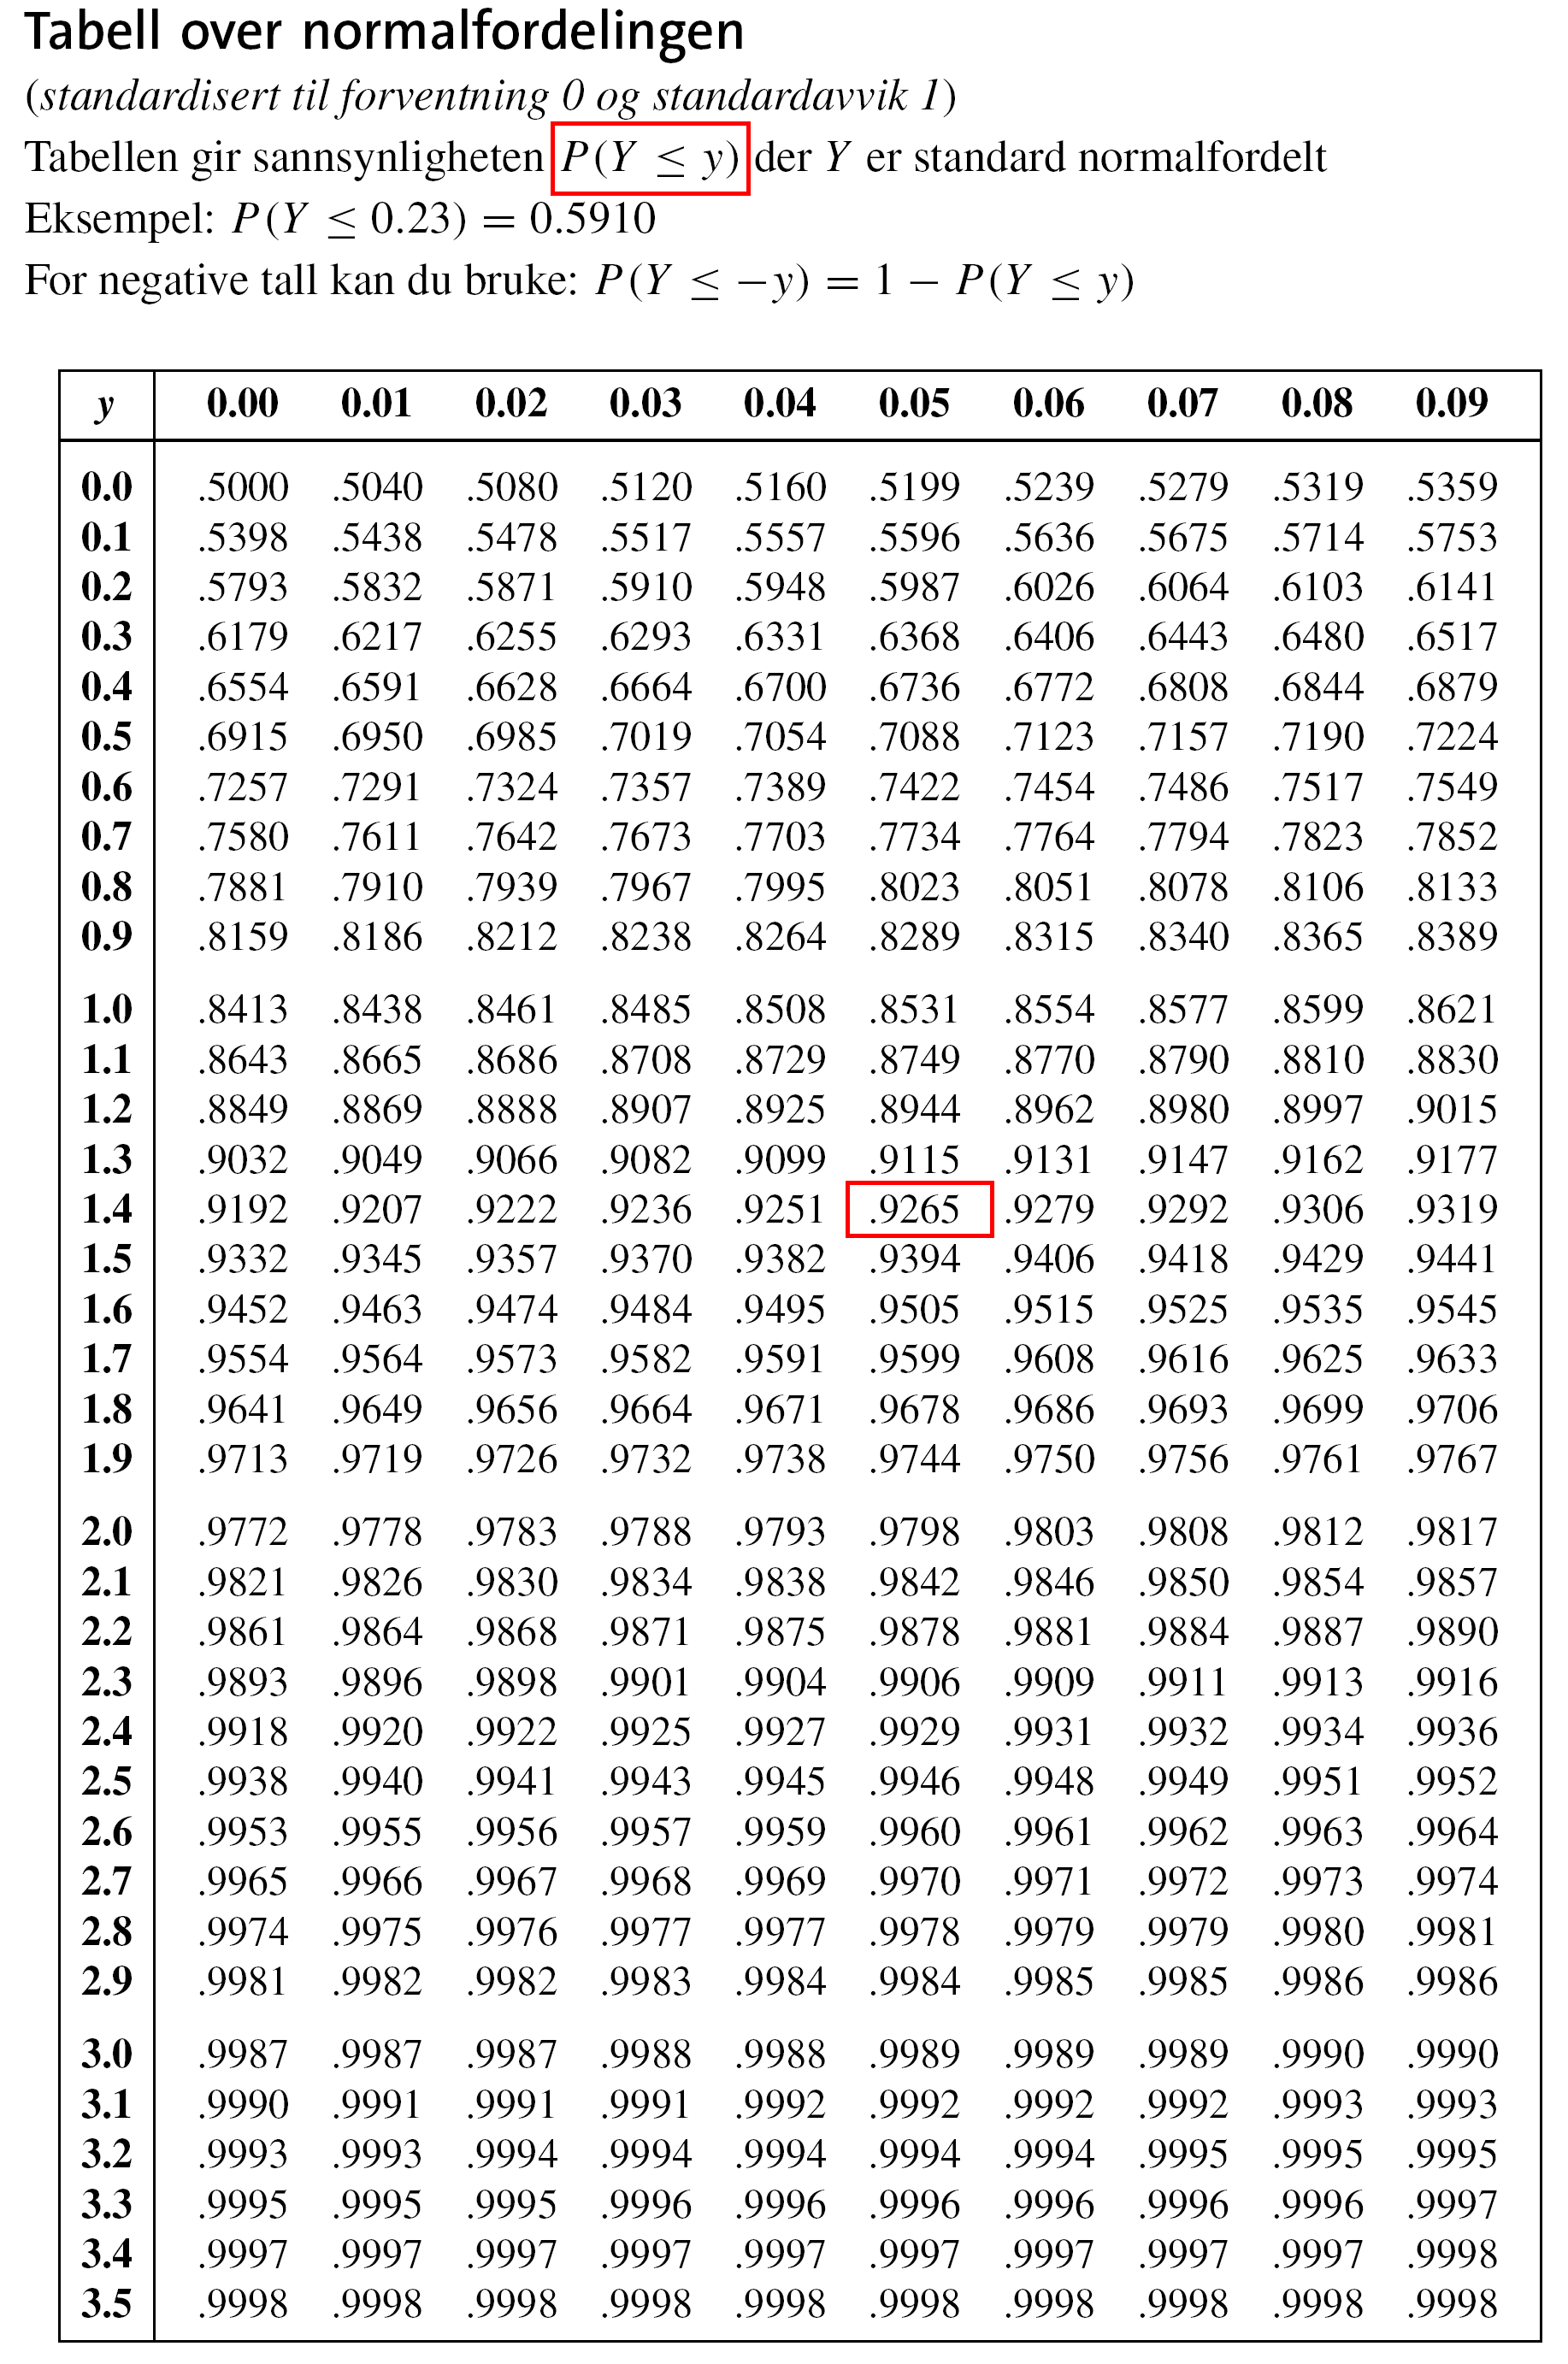
\includegraphics[height=0.9\textheight]{normaltina4.png}
      %\caption{}
    \end{center}
  \end{figure}
}

\frame{ 
\frametitle{}
  \begin{block}{}
    \begin{itemize}
    \item P(X > 4000) = 1 - P(X $\leq$ 4000) = 1 -
      P($\frac{X-2945}{729} \leq 1.45$) \vspace{0.3cm} \\ \hspace{2.1cm} = 1 - 0.9265 = 0.0735
      $\approx$ 7\%
     \end{itemize}
  \end{block}
\pause
  \begin{block}{Pay attention}
    \begin{itemize}
    \item The normal distribution table shows different probabilities:
    \begin{itemize}
    \item Aalen: P(Y $\leq$ y)   
    \item Kirkwood: P(Y \hl{$\geq$} y)
     \end{itemize}
     \end{itemize}
  \end{block}
}

\frame{ 
\frametitle{The normal approximation to the Binomial distribution}
  \begin{block}{Remember the Binomial:}
    \begin{itemize}
    \item $P(X = x) = \binom{n}{x} p^x (1-p)^{n-x}$, \\ \vspace{3mm}
      
      where $\binom{n}{x} = \frac{n \cdot (n-1) \cdot ... \cdot (n - x
        +1)}{1 \cdot 2 \cdot ... \cdot x}$ and $\binom{n}{0} = 1$
     \end{itemize}
  \end{block}
  \begin{block}{Solution for large $n$}
    \begin{itemize}
    \item Use the normal distribution!
     \end{itemize}
  \end{block}
}

\frame{ 
\frametitle{The normal approximation to the Binomial distribution}
  \begin{block}{Remember this morning:}
    \begin{center}
      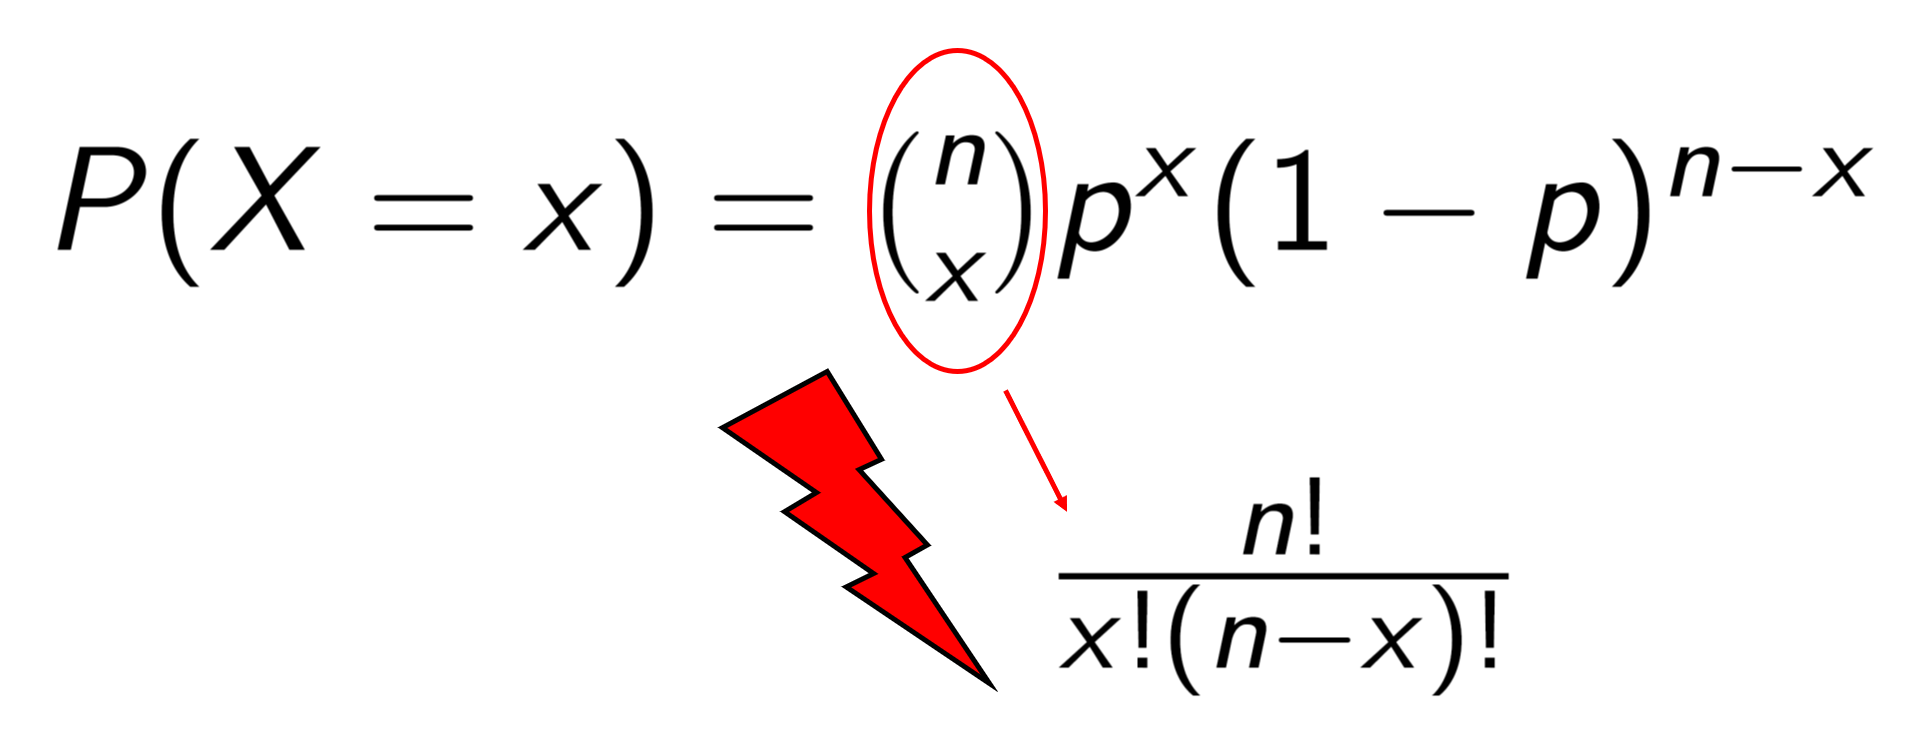
\includegraphics[height=0.35\textheight]{normal3modified.png}
    \end{center}
  \end{block}
  \begin{block}{Solution for large $n$}
    \begin{itemize}
    \item Use the normal distribution!
     \end{itemize}
  \end{block}
}

%% \frame{
%% \frametitle{}
%% \begin{block}{}
%%   \begin{figure}[ht]
%%     \begin{center}
%%       \includegraphics[height=0.82\textheight]{Figur5-5.png}
%%       %\caption{}
%%     \end{center}
%%   \end{figure}
%% \end{block}
%% }

\frame{
\frametitle{}
\begin{block}{Histograms of Binomial distributions with $p = 0.2$}
  \begin{figure}[ht]
    \begin{center}
      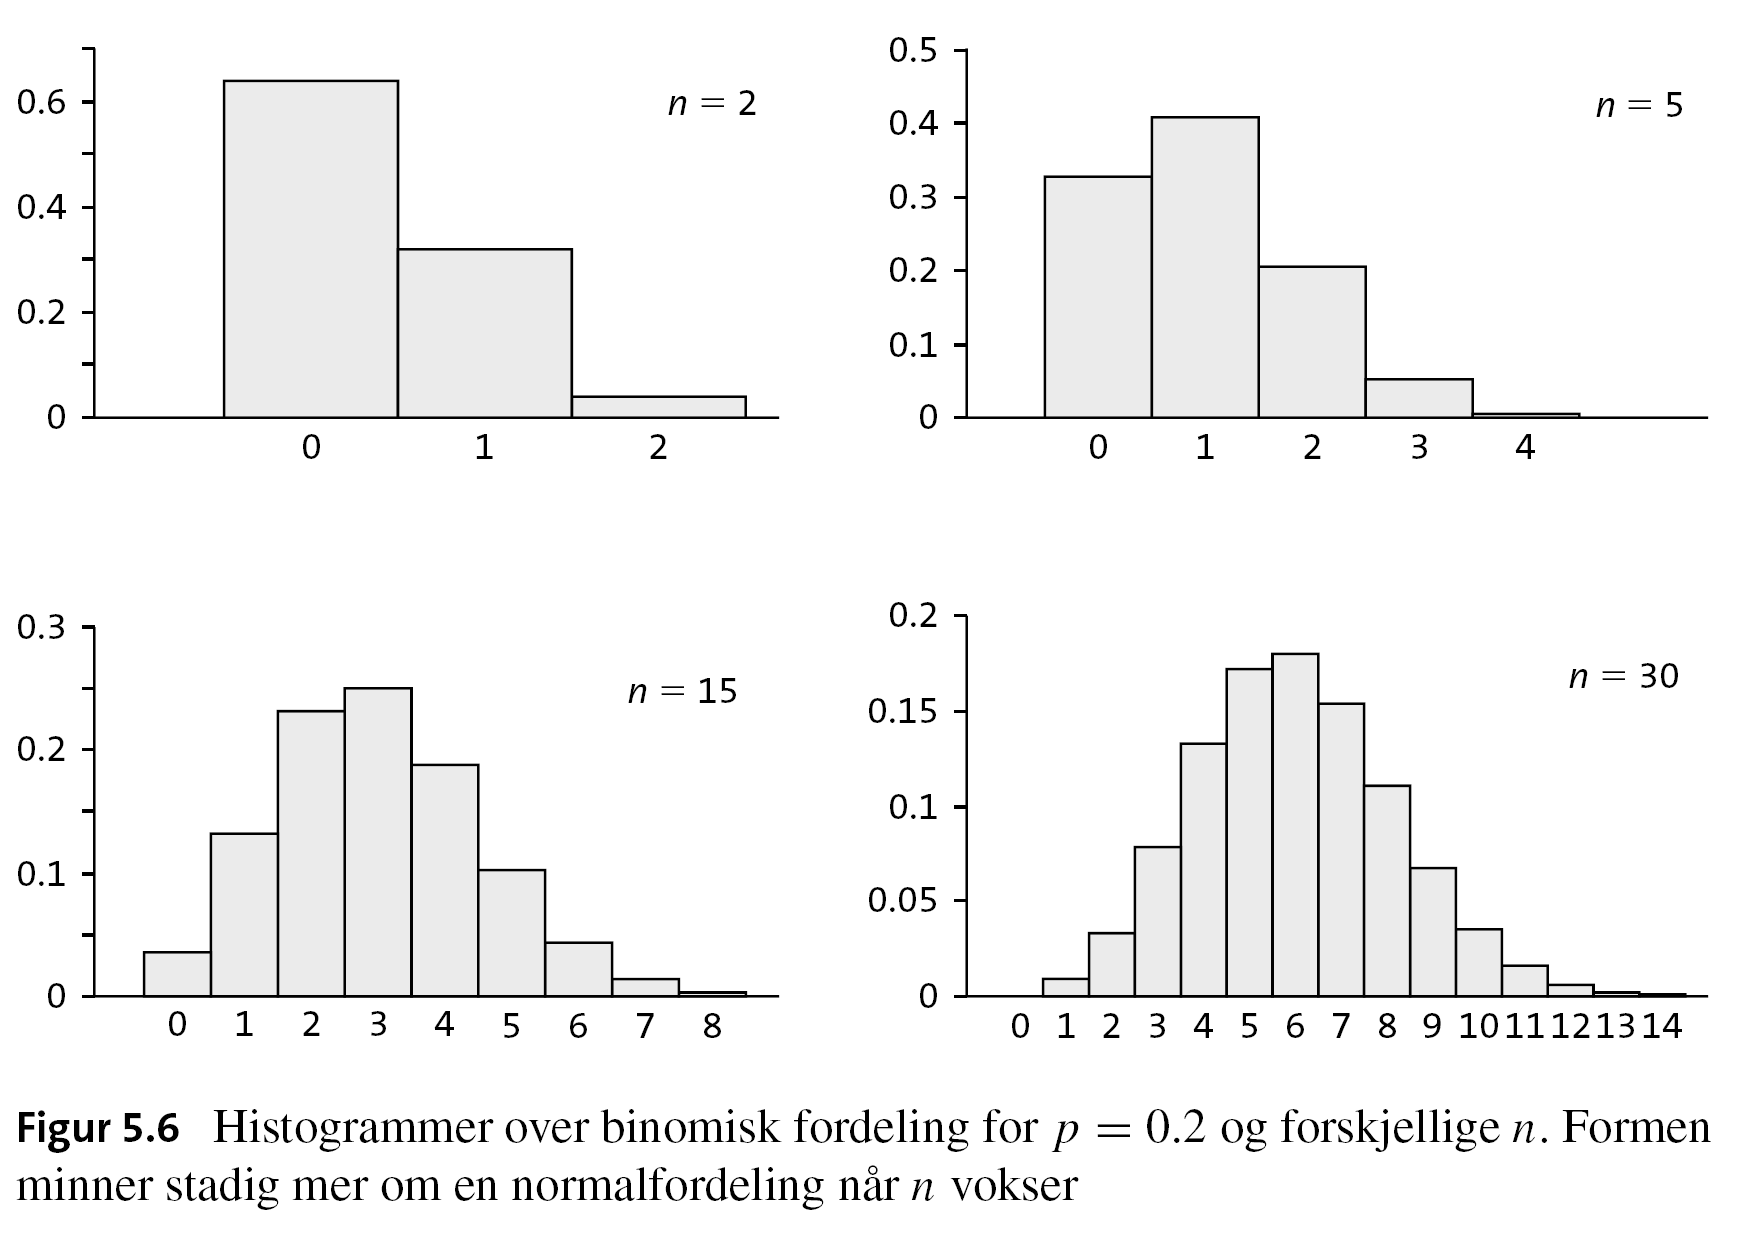
\includegraphics[height=0.70\textheight]{Figur5-6.png}
      %\caption{}
    \end{center}
  \end{figure}
    \begin{itemize}
    \item Observe how the shape of the distributions becomes more and
      more similar to a normal distribution when we increase $n$
     \end{itemize}
\end{block}
}

\frame{ 
\frametitle{}
  \begin{block}{Fitting a normal distribution to  approximate a Binomial distribution}
    \begin{itemize}
    \item $\mu = np$
    \item $\sigma = \sqrt{np(1-p)}$
     \end{itemize}
  \end{block}
}

\frame{
\frametitle{}
\begin{block}{Example: number of boys out of 20 newborns}
    \begin{itemize}
    \item $n = 20$, $p = 0.514$
    \item $\mu = np = 20 \cdot 0.514 = 10.28$
    \item $\sigma = \sqrt{np(1-p)} = \sqrt{20 \cdot 0.514 \cdot 0.486} = 2.24$ $\rightarrow$ N(10.28, 2.24)
     \end{itemize}
  \begin{figure}[ht]
    \begin{center}
      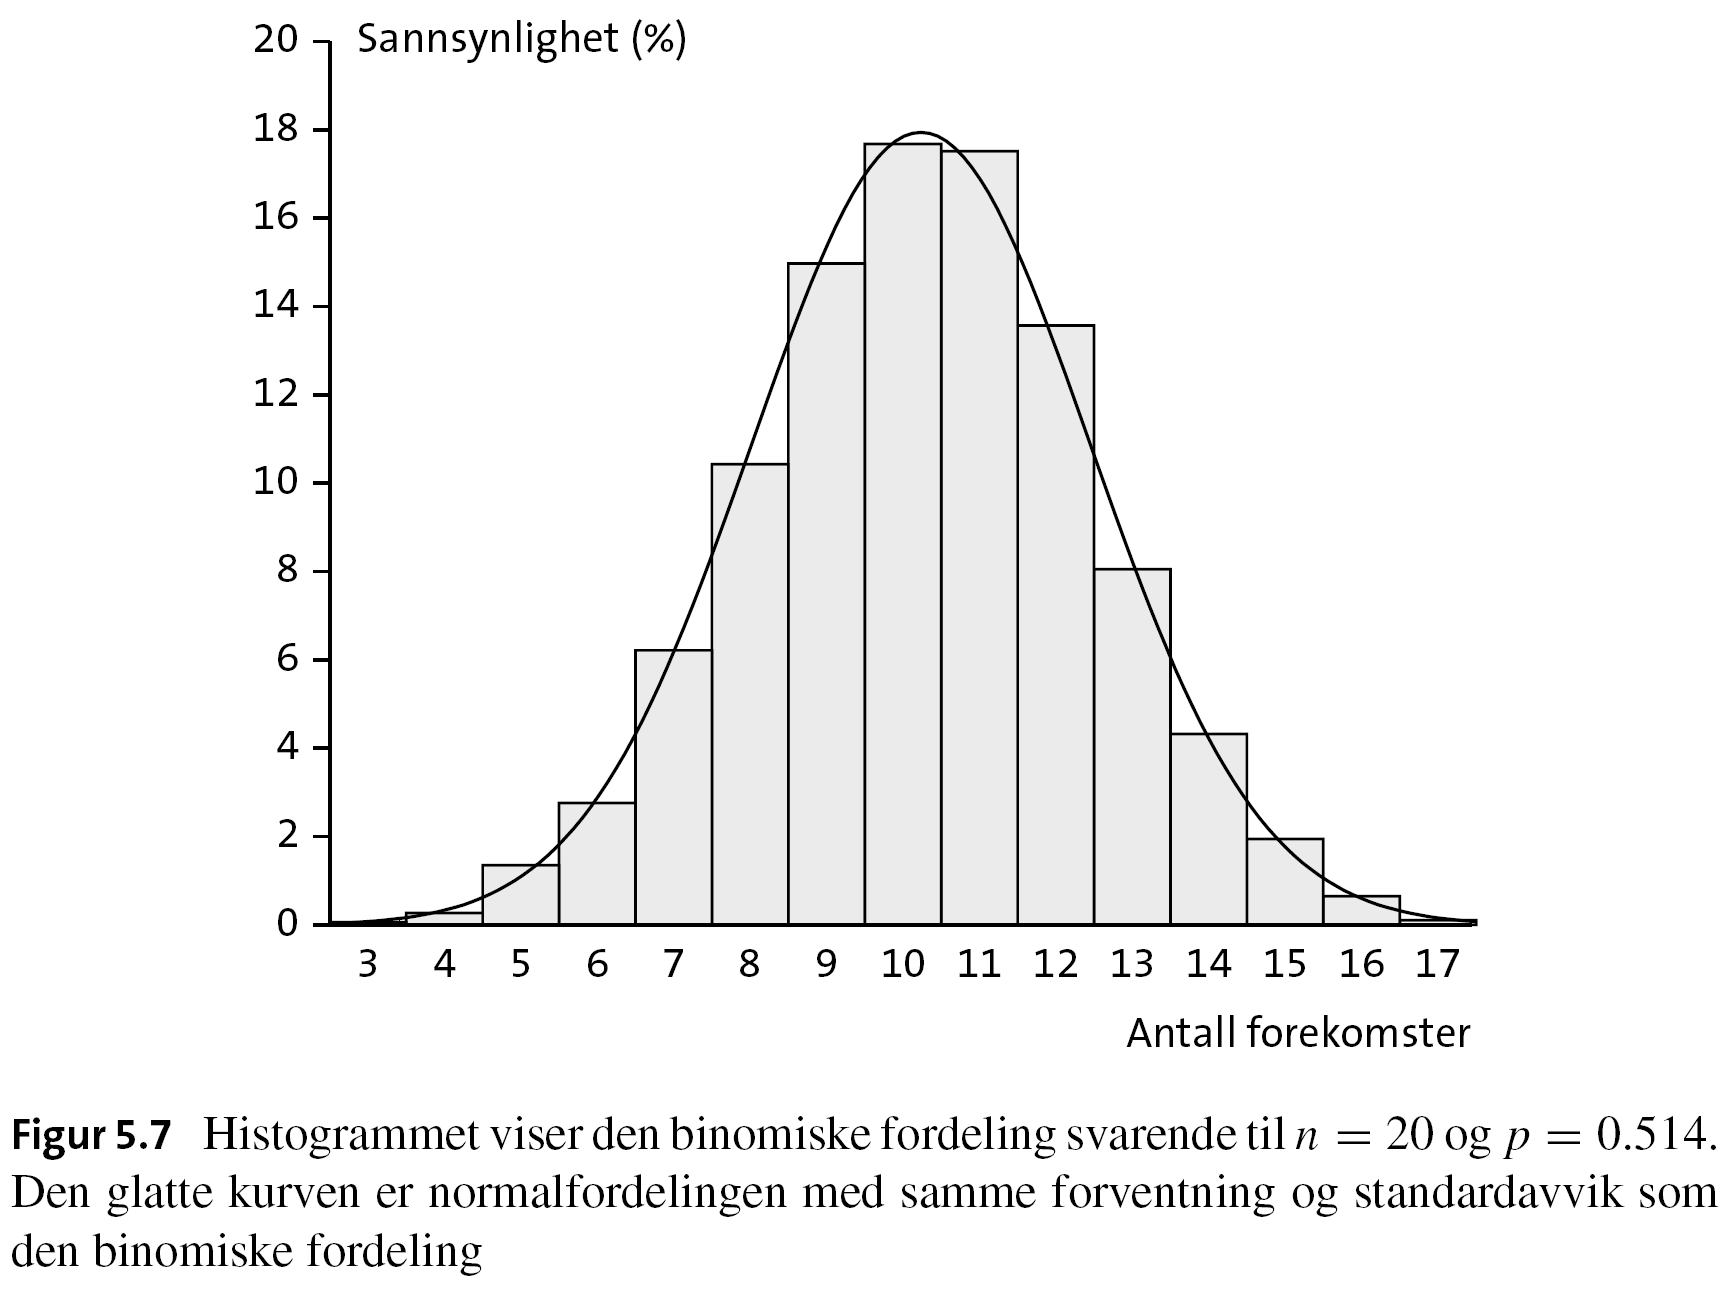
\includegraphics[height=0.60\textheight]{Figur5-7.png}
      %\caption{}
    \end{center}
  \end{figure}
\end{block}
}

\frame{ 
\frametitle{}
  \begin{block}{Approximation}
    \begin{itemize}
    \item B($n$,$p$) $\rightarrow$ N($\mu, \sigma$) for $n \rightarrow \infty$
    \item Rule: ... if $np \geq 5$ and $n(1-p) \geq 5$
    \item Theory: \hl{the central limit theorem} (easy version, in words)
    \begin{itemize}
    \item \emph{The distribution of the sample means will be nearly normal
      whatever the distribution of the variable in the population is -
      as long as the samples are large enough}
     \end{itemize}\pause
   \item Remark: remember that the observed proportion (e.g. relative
     frequency of boy-births) can be considered to be a mean!
     \end{itemize}
  \end{block}
}


\section{Summary}

\frame{ 
\frametitle{Summary}
  \begin{block}{Key words}
    \begin{itemize}
    \item (Continuous) Probability distributions
    \item Continuous variables
    \item The normal distribution
    \item Location and variation
    \item The standard normal distribution
    \end{itemize}
  \end{block}
  \begin{block}{Notation}
    \begin{itemize}
   \item $f(x)$
    \item $\mu$, $\sigma$
     \item N($\mu$,$\sigma$)
    \item N(0,1)
    \end{itemize}
  \end{block}
}

\end{document}

